\documentclass{sig-alternate}

\usepackage{amsmath,amssymb,amsfonts,amsmath}
\usepackage{hyperref}
\usepackage{color}
\usepackage{comment}
\usepackage{mdwlist}

\includecomment{mycomment}

%%%%%%%%%%%%%%%

\newcommand{\ff}[1]{\mathbb{F}_{#1}}
\newcommand{\fq}{\ff{q}}
\newcommand{\fqn}{\ff{q^n}}

\newcommand{\dd}{d}
\newcommand{\qq}{q}
\newcommand{\nn}{n}
\newcommand{\qn}{{\qq^\nn}}
\newcommand{\extfactfdegree}{k}
\newcommand{\extfactfsize}{\qq^{\nn \cdot \extfactfdegree}}

% if we define everything in terms of base field, extension field and
% extension field used in factorization
\newcommand{\basef}{\ff{\qq}}
\newcommand{\extf}{\ff{\qn}}
\newcommand{\extfactf}{\ff{\extfactfsize}}

\DeclareMathOperator{\Tr}{Tr}
\DeclareMathOperator{\Ker}{Ker}
\DeclareMathOperator{\Ima}{Im} 
\DeclareMathOperator{\Decomp}{Decomp} 

% to specify the number of elements of the finite fields on which the
% trace is defined
\newcommand{\tr}[2]{\Tr_{\ff{#1}:\ff{#2}}}

% to specify the number of elements of the finite fields on which the
% trace is defined: light form
\newcommand{\trl}[2]{\Tr_{#1:#2}}

% to specify the notation of the finite fields on which the trace is
% defined
\newcommand{\trabs}[2]{\Tr_{#1:#2}}
\newcommand{\trextbase}{\trabs{\extf}{\basef}}
\newcommand{\trextfactext}{\trabs{\extfactf}{\extf}}
\newcommand{\trextfactbase}{\trabs{\extfactf}{\basef}}

\newcommand{\bigO}{O}
\newcommand{\bigOt}{\tilde{O}}
\newcommand{\smallO}{o}
\newcommand{\Mul}{\mathsf{M}}

\newcommand{\Span}{\mathbf{span}}
\newcommand{\card}[1]{\# #1}
\DeclareMathOperator{\Res}{Res}

\newcommand{\cost}[1]{\color{blue}Cost:  #1\color{black}}

%%%%%%%%%%%% Algorithms

\usepackage{float,algorithm}
\usepackage[noend]{algorithmic}
\renewcommand{\algorithmicrequire}{\textbf{Input:}}
\renewcommand{\algorithmicensure}{\textbf{Output:}}

\newcounter{algo}

\newenvironment{algorithm_noendline}[4]{\begin{center}\begin{minipage}{0.48\textwidth}
      \refstepcounter{algo}
      \label{#4}
      \sf
      \rule{\textwidth}{0.2pt}\\
      \makebox[\textwidth][c]{Algorithm~\arabic{algo}:~\textbf{#1}}\\
      \rule[0.5\baselineskip]{\textwidth}{0.2pt}\\

      \vspace{-12pt}

      \parbox{\textwidth}{\textbf{Input} #2}
      \parbox{\textwidth}{\textbf{Output} #3}

\vspace{-7pt}

      \begin{enumerate*}}{\end{enumerate*}
      \vspace{-11pt}
\end{minipage}\end{center}
}

\newenvironment{algorithm_endline}[4]{\begin{center}\begin{minipage}{0.48\textwidth}
      \refstepcounter{algo}
      \label{#4}
      \sf
      \rule{\textwidth}{0.2pt}\\
      \makebox[\textwidth][c]{Algorithm~\arabic{algo}:~\textbf{#1}}\\
      \rule[0.5\baselineskip]{\textwidth}{0.2pt}\\

      \vspace{-12pt}

      \parbox{\textwidth}{\textbf{Input} #2}
      \parbox{\textwidth}{\textbf{Output} #3}

\vspace{-7pt}

      \begin{enumerate*}}{\end{enumerate*}
      \vspace{-11pt}
      \rule{\textwidth}{0.2pt}
\end{minipage}\end{center}
%\vspace{-0.5cm}
}

\floatstyle{plain}
\newfloat{algofloat}{thp}{bla}
\floatname{algofloat}{}

%%%%%%%%%%

\newcommand{\todo}[1]{\textcolor{red}{TODO: #1}}
\newcommand{\com }{\noindent \textcolor{blue}{Commentaire Micha\"el}:}
\newcommand{\comd}{\noindent \textcolor{blue}{D\'ebut Micha\"el}:}
\newcommand{\comf}{\noindent \textcolor{blue}{:Fin Micha\"el}}




\newtheorem{Def}{Definition}
\newtheorem{Theo}{Theorem}
\newtheorem{Prop}{Proposition}
\newtheorem{Lem}{Lemma}
\newtheorem{Coro}{Corollary}

\renewcommand{\paragraph}[1]{\smallskip\noindent{{\bf \rm #1.}}}

\numberofauthors{3}
\author{
  \alignauthor Luca De Feo\\
  \affaddr{Laboratoire PRiSM}\\
  \affaddr{Universit\'e de Versailles}\\
  \email{luca.de-feo@uvsq.fr}
  \alignauthor Christophe Petit\\
  \affaddr{Crypto Group}\\
  \affaddr{University College London}\\
  \email{}
  \alignauthor Micha\"el Quisquater\\
  \affaddr{Laboratoire PRiSM}\\
  \affaddr{Universit\'e de Versailles}\\
  \email{mquis@prism.uvsq.fr}
}

\title{Deterministic root finding in small characteristic finite
  fields}

\begin{document}


\maketitle
\begin{abstract}
  The resolution of polynomial equations over finite fields has many
  applications, for example in cryptography or coding theory. Starting
  from the work of Berlekamp in the eighties, many efficient
  algorithms have been proposed to solve this problem faster, either
  asymptotically or in practice.  In this paper, we consider the case
  of polynomials over $\fqn$ where $\qq$ is a small number. We propose a
  new algorithm to solve this problem, merging features of Berlekamp's
  classical trace algorithm (BTA) and the recent successive resultant
  algorithm (SRA).  Similarly to BTA, our algorithm separates the
  roots of the polynomial into distinct subspaces using gcd
  computations. Similarly to SRA, it uses particular subspaces that
  are embedded in one another.

  Our algorithm has an asymptotic complexity similar to BTA and SRA on
  this type of polynomials ... It has this and this great advantages
  over these algorithms. Our Sage implementations show that it is
  great, easy to implement, very efficient, and beat previous
  algorithms on a large range of parameters...

  We also provide optimizations and a factorization version of our
  algorithm that are of further interest for SRA.
\end{abstract}

\category{F.2.1}{Theory of computation}{Analysis of algorithms and problem complexity}[Computations in finite fields]
\category{G.4}{Mathematics of computing}{Mathematical software}
\terms{Algorithms,Theory}
\keywords{Finite fields, root finding, factoring.}

%%%%%%%%%%%%%%%%%%%%%%%%%%%%%%%%%%%%%%%%%%%%%%%%%%%%%%%%%%%%
%%%%%%%%%%%%%%%%%%%%%%%%%%%%%%%%%%%%%%%%%%%%%%%%%%%%%%%%%%%%
%%%%%%%%%%%%%%%%%%%%%%%%%%%%%%%%%%%%%%%%%%%%%%%%%%%%%%%%%%%%


\section*{Notations: to remove at the end of the writing}


\noindent {\bf Finite field:}
\begin{itemize}
\item $\ff{p}$: generic form
\item $\fq$: base field 
\item  $\fqn$ : extension field  
\end{itemize}

\medskip

\noindent {\bf Abstract notation for fields}

\begin{itemize}
\item $K$: $\basef$: base field
\item $L$:  $\extf$: extension field 
\item $E$: $\extfactf$ : field extension of $L$ with degree $k$  
\item $\qq$
\item $\qn$
\item $\extfactfsize$ : useless if we don't speak about factorization
\item $\nn$ : 
\item $\extfactfdegree$ : useless if we don't speak about factorization

\end{itemize}




\medskip


\noindent {\bf Trace map on finite fields:}

\begin{itemize}
\item $\tr{p^n}{p}(X)$: generic form
\item $\trl{p^n}{p}(X)$: generic light form
\item $\trabs{L}{K}(X)$: generic abstract form
\item $\trextbase(X)$ :trace from the extension field to its base field 
\item $\trextfactext(X)$ : useless if we don't speak about factorization
\item $\trextfactbase(X)$ : useless if we don't speak about factorization

\end{itemize}


\noindent {\bf Complexity of computation in finite fields:}

Ideally we should express everything in term of the cost of a multiplication in  a finite field.

\begin{itemize}
\item $\Mul(n)$: cost of polynomial multiplication
\item Distinguish conventional arithmetic and fast arithmetic. Reuse the tables of \cite{KaltofenS97} or \cite{Umans08}.
\end{itemize}




\section{Introduction}

This paper presents and compares two related algorithms for finding
roots of polynomials with coefficients in a finite field $\extf$,
where $\qq$ is small. The first algorithm, called the Successive
Resultants Algorithm (SRA), was already introduced by C.~Petit
in~\cite{cgUCL-P14}. We give here a fresh look at it and show how it
is related to the second one. The second algorithm, called the Affine
Refinement Method (ARM), is new, and similar in spirit to Berlekamp's
Trace Algorithm (BTA)~\cite{berl70}.

Both algorithms are deterministic. They find all the roots of a
square-free, split polynomial of degree $\dd$ using \todo{} operations
over $\basef$ in the worst case, and an expected \todo{} on
average. Hence, they improve over previously known deterministic
algorithms for root finding~\cite{Shoup91b} \todo{do they?}. For some
parameter ranges, they also compare favorably in practice with the
best randomized algorithms for root finding~\cite{berl70,cantor1981}.

Any algorithm for root finding can be extended to an algorithm for
factoring polynomials as mentioned in~\cite{Rabin79}. Doing so with
our algorithms does not improve over the previous literature
\todo{unless it does?}. However we argue in
Section~\ref{sec:factorization} that a partial application of this
idea yields a practical improvement to the classical Cantor-Zassenhaus
algorithm~\cite{cantor1981}.

\paragraph{Previous work} 

\paragraph{Our contribution}

\paragraph{Outline}


\section{Background and Notation}

We are interested in algorithms for the following problem: given a
degree $\dd$ polynomial $f(X)$ with coefficients in a finite field
$\extf$, find all the roots $\rho\in\extf$ such that $f(\rho)=0$.  

\paragraph{Complexity notations} In this paper, we use an
\emph{algebraic complexity model}, where the running time of an
algorithm is measured in terms of the number of operations ($+$,
$\times$, $\div$) in $\extf$, and its space requirements in terms of
number of elements of $\extf$ stored. As customary, we use the
$\bigO$-notation to neglect constant factors, and the
$\bigOt$-notation to further neglect poly-logarithmic factors. All
asymptotic complexities will be expressed in terms of the parameters
$\qq$, $\nn$ and $\dd$.

We denote by $\Mul : \mathbb{N} \to \mathbb{N}$ a function such that
polynomials in $\extf[X]$ of degree at most $m$ can be multiplied in
$\Mul(m)$ operations ($+$, $\times$) in $\extf$, and we make the
usual super-linearity assumptions on
$\Mul$~\cite[Chapter~8]{Gathen2003}.  Using FFT multiplication, we can
take $\Mul(m)\in\bigOt(m)$.


\subsection{Nested subspace decomposition of $\extf$}
\label{sec:nsd}

We now present the main ingredient of our algorithms. It consists in a
decomposition of the $\basef$-vector space $\extf$ into a sequence of
nested affine subspaces.

\paragraph{Approximating $\extf$ by a flag} Let
$\{\upsilon_1,\ldots,\upsilon_\nn\}$ be any basis of $\fqn/\fq$ (not
necessarily the one used to represent the elements of $\extf$). To
this basis, we associate the flag of linear subspaces $V_0\subset
V_1\subset \cdots \subset V_\nn$ defined by
\begin{equation}
  V_i = \Span(\upsilon_1,\dots,\upsilon_i),
\end{equation}
so that $\dim V_i = i$ and $\card V_i = \qq^i$. To each of the
subspaces we associate its minimal polynomial, that we denote by
$L_i$. Then we have the well know relation (see
\cite[Lemma~1]{cgUCL-P14})
\begin{equation}
  L_0(X) = X, \quad L_i(X) = (X^\qq - L_{i-1}(\upsilon_i)^{\qq-1}X)\circ L_{i-1}(X),
\end{equation}
where we remark that the $L_i$'s are linearized polynomials (see
\cite[Ch. 11]{Berlekamp1984}), and in particular $L_\nn=X^\qn-X$.

Notice that, by definition, each $L_i$ defines a linear map
$\extf\to\extf$, with kernel $V_i$. It will be convenient to encode
this information in an $\nn\times\nn$ matrix, thus we define
$\gamma_{i,j}=L_i(\upsilon_j)$, and
\begin{equation}
  \label{eq:Gamma}
  \Gamma =
  \begin{pmatrix}
    \gamma_{0,1} & \cdots & \gamma_{0,\nn}\\
    \vdots & & \vdots\\
    \gamma_{\nn-1,1} & \cdots & \gamma_{\nn-1,\nn}
  \end{pmatrix}.
\end{equation}
Observe that by definition $\gamma_{i,j}=0$ whenever $j\le i$, hence
$\Gamma$ is an upper triangular matrix, associated to a linear map
$\extf\to\extf^\nn$ sending any $\delta\in\extf$ to the vector
$L_0(\delta),\dots,L_{n-1}(\delta)$.  
\comd
 Il doit manquer un last quelque part.
\comf
We finally define $V_i^\ast$ as
the image space of $L_i$, i.e. the subspace generated by the $i$-th
row of $\Gamma$.  It is easily verified that $\dim V_i^\ast=n-i$ and
that $\{\gamma_{i,i+1},\dots,\gamma_{i,\nn}\}$ is a basis.

\comd
Let us define the dual of $L_i$, denoted by $L_i^\ast$, as the unique linearized polynomial (see
\cite[Ch. 11]{Berlekamp1984}) such that 
$$(L_i^\ast \circ L_i)(X)=(L_i^\ast \circ L_i)(X)=X^\qn-X\,.$$
In particular, $L_i^\ast(L_i(\alpha))=0$ for any $\delta \in \extf$. Therefore, $V_i^\ast=\Ker L_i^\ast=\Ima~L_i$.
\comf


\begin{Lem}
  The coefficients of the matrix $\Gamma$ can be computed using
  $O(\nn^2\log\qq)$ operations over $\extf$.
\end{Lem}
\begin{proof}
  By the recursive definition of $L_i$, it is clear that
  \begin{equation}
    \gamma_{i,j} =
    \begin{cases}
      \upsilon_j &\text{for $i=0$},\\
      \gamma_{i-1,j}^\qq - \gamma_{i-1,i}^{\qq-1}\gamma_{i-1,j} &\text{for $i>0$}.
    \end{cases}
  \end{equation}
  Thus, each $\gamma_{i,j}$ can be computed from the previous ones
  using $O(\log\qq)$ operations, and there is a total $O(\nn^2)$ of
  them to compute.
\end{proof}

The eigenvalues of $\Gamma$ play a special role in our algorithms,
thus we define $\beta_i=\gamma_{i-1,i}$ and $\alpha_i=\beta_i^{\qq-1}$
for any $1\le i \le \nn$. We deduce a decomposition
\begin{equation}
  X^\qn - X = (X^\qq - \alpha_\nn X) \circ \cdots \circ (X^\qq - \alpha_1 X).
\end{equation}

\paragraph{Covers of $\extf$ by affine subspaces} We now build a
sequence of covers of $\extf$ by affine subspaces, each one being a
subcover of the next one.

Let now $\rho\in\extf$, such that $\rho=\sum_jr_j\upsilon_j$.  For any
$V_i$ we define the affine space
\begin{equation}
  V_{i,\rho} = V_i + \rho.
\end{equation}
We also define the polynomial $M_{i,\rho}$ as the minimal polynomial
of $V_{i,\rho}$, hence
\begin{equation}
\label{node_product}
  M_{i,\rho}(X) = L_i(X - \rho) = L_i(X) - \sum_{j>i}r_j\gamma_{i,j}.
\end{equation}
Observe that $M_{i,\rho}=M_{i,\rho'}$, and thus
$V_{i,\rho}=V_{i,\rho'}$, if and only if $\rho-\rho'\in V_i$. Hence
there are exactly $\qq^{n-i}$ distinct affine spaces of the form
$V_{i,\rho}$, each of size $\qq^i$.

By definition we have
\begin{equation}
  V_{i,\rho} = \bigcup_{c\in\basef} V_{i-1,\rho + c\upsilon_i},
\end{equation}
hence
\begin{equation}
  M_{i,\rho}(X) = \prod_{c\in\basef} M_{i-1,\rho+c\upsilon_i}(X).
\end{equation}
Thus for each $i$, the distinct $V_{i,\rho}$'s form a cover of
$\extf$, and the $V_{i-1,\rho}$'s form a subcover of the $V_{i,\rho}$,
with $V_{i-1,\rho}\subset V_{i,\rho'}$ if and only if $\rho-\rho'\in
V_{i-1}$.  We deduce a sequence of factorizations of $X^\qn-X$ as
follows
\begin{equation}
  \label{eq:product-tree}
  \begin{gathered}
    X^\qn-X = M_{n,0}(X) =
    \prod_{c_1\in\basef}M_{n-1,c_1\upsilon_n}(X)=\\
    \prod_{c_1,c_2\in\basef}M_{n-2,c_2\upsilon_{n-1}+c_1\upsilon_n}(X)=\\
    \cdots=\\
    \prod_{c_1,\dots,c_n\in\basef}M_{0,c_n\upsilon_1+\cdots+c_1\upsilon_n}(X)=
    \prod_{\rho\in\extf}(X-\rho),
  \end{gathered}
\end{equation}
where the last equality comes from the fact that $L_0$ is the identity
map.

\comd
Let us finally remind some well-known facts about resultants.
Consider the polynomial $f \in \extf[X]$ and the projections $P_1, P_2 \in  \extf[X]$ and define $P$ as $P_2 \circ P_1$.
According to the property about the root's of resultants,
$$g(Y)=\Res_X(f(X),P(X)-Y)=\prod_{\{\rho \mid f(\rho)=0\}} (P(\rho)-Y) \,.$$
Therefore, the roots of the resultant $g(Y)$ are the projection of the roots of $f(X)$ throught $P$.
Also, 
\begin{equation}
\label{resultant_compose}
g(Y)=\Res_{Y_1}(g^{(1)}(Y_1),Y-L_2(Y_1))
\end{equation}
 where $g^{(1)}(Y_1)=\Res_{Y}(f(X),Y_1-L_1(X))$. Finally, 
 the algebraic multiplicity of a root of $g$ is the number of roots of $f$ projected to this root.
\comf



\paragraph{Application to root finding} From the objects we have
defined so far, we derive two algorithms for computing the roots of a
polynomial $f$ with coefficients in $\extf$. Both algorithms are
iterative in nature and work by ascending/de\-scend\-ing along the
flag $V_0,\dots,V_n$. In an abstract way, they can be seen as
\emph{dual} to each other.

SRA transforms $f$ by \emph{projecting} its roots onto the spaces
$V_i^\ast$.  Starting from the polynomial $f_0=f$ with roots in
$V_0^\ast=\extf$, we iteratively compute polynomials $f_1,\dots,f_n$
such that the roots of $f_i$ are the projections onto $V_i^\ast$ of
the roots of $f_{i-1}$.  The successive projections are computed by
means of resultants.  Ultimately, $f_n$ will have $0$ as only root,
and the original roots will be found by ascending the chain back to
$f_0$.  Said otherwise, for any root $\rho$ of $f$, SRA computes
successive approximations $L_n(\rho),L_{n-1}(\rho),\dots,L_0(\rho)$,
ultimately yielding the original root because $L_0(\rho)=\rho$.

On the other hand, ARM isolates the roots of $f$ by
\emph{intersecting} them with the subspaces $V_{i,\rho}$, starting
from the largest space $V_{n,0}$, and iteratively going down to the
smallest ones $V_{0,\rho}$.  The successive intersections are computed
by means of GCDs.  Said otherwise, for any root $\rho=\sum_j
r_j\upsilon_j$ of $f$, ARM computes successive approximations
$\rho_k=\sum_{j>k}r_j\upsilon_j$, from $\rho_n=0$ down to
$\rho_0=\rho$.


\comd
{\bf }La vision n'est pas la m\^eme que ci-dessus ("application to root finding") mais ce n'est pas en contradiction. J'ai essay\'e de faire un mais mais ce n'est pas complet. De mon point de vue la notion d'approximation ne vient que lorsque l'on instantie les espaces $V_i$ et $V_i^\ast$. A partir des coefficients $r_i$, on peut calculer les $\sum_{i<j} r_i \upsilon_i$.

\section{Preliminaries}

In this section we review the fundamental subroutines upon which are
going to be based the algorithms of the next sections.

\todo{Do we need to remind the costs of:
  \begin{itemize}
  \item gcd?
  \item square-free factorization?
  \item ddf?
  \item modular composition?
  \item iterated frobenius and similar tricks?
  \item multipoint evaluation / interpolation?
  \end{itemize}
}

\begin{Lem}
  Let $f$ be a polynomial in $\extf$ of degree $\dd\gg\qq$. Let
  $\delta_0,\dots,\delta_\dd\in\extf$ be a list of evaluation points,
  and let $\beta\in\extf$.  All the values
  \begin{equation*}
    f(\delta_i + c\beta) \qquad\text{for any $0\le i\le d$ and any $c\in\basef$}
  \end{equation*}
  can be computed using $O(\Mul(\dd) \log_\qq\dd +
  \qq^2\Mul(\dd/\qq)\log\dd + \qq^2\dd)$ operations over $\extf$.
\end{Lem}
\begin{proof}
  \todo{(Luca) See Python code. Note: this is a minor gain, compared
    to a classic multi-point evaluation (which would cost
    $O(\qq\Mul(d)\log d)$), but it is a gain, and it even is
    practical, thus we may leave this if we have space.}
\end{proof}

\begin{Lem}
  Let $f$ be a polynomial in $\extf$ of degree $d<\qq^{\nn-1}$, and
  let $\beta\in\extf$. The resultant
  \begin{equation*}
    \Res_X(f(X), Y-X^\qq+\beta^{\qq-1} X)
  \end{equation*}
  can be computed using $O(\Mul(\dd) \log\dd +
  \qq^2\Mul(\dd/\qq)\log\dd + \qq^2\dd)$ operations over $\extf$.
\end{Lem}
\begin{proof}
  \todo{(Luca or whoever feels like writing it) This one's easy: its
    just one application of the previous lemma, plus the cost of one
    interpolation $O(\Mul(d)\log d)$}
\end{proof}



\section{Link between ARM and SRA}
\label{sec:arm-sra}

In this section we show that ARM and SRA methods can be seen as
\emph{dual} to each other if we remember that
$$\gcd(f(X),g(X)) \ne 1 \mbox{  if and only if }\Res_X(f(X),g(X))=0\,.$$

\medskip

\noindent {\bf Pre-computation}: Both methods, ARM and SRA, start by computing the decomposition of the field equation following the procedure described in relation~(\ref{Li_generation}), i.e.
 $$X^{\qn}-X=(X^\qq - \alpha_\nn) \circ (X^\qq - \alpha_{\nn-1}) \circ \cdots \circ (X^\qq - \alpha_1) \,.$$
where $\alpha_i \in \extf$. This determine in particular the different linearized polynomials $L_i$ and the spaces $V_i=\Ker~L_i$ and $V_i^\ast=\Ima~L_i$. Note that this phase depends only on the field and may be re-used for the root-finding of several polynomials $f \in \extf[X]$ defined on the same field.

\medskip

\noindent {\bf ARM}: The method consists in \emph{projecting} the roots of $f$ onto the spaces $V_i^\ast$ while simultaneously \emph{intersecting} those with the corresponding fibers of $L_i$ identified by $\ell_i$.
 It is achieved by the computation of the minimal polynomial of those intersections by means of gcd's, i.e. 
 \begin{equation}
 \label{base_ARM}
\gcd(f(X),L_i(X)-\ell_i)     \mbox{ for any }  \ell_i  \in V_i^\ast\,,
\end{equation}
for $i$ starting from $n$ and going down to 0.
It will anyway leads to the root of $f$ because 
$$\gcd(f(X),L_0(X)-\ell_0)=\gcd(f(X),X-\ell_0) \ne 1\,,$$ 
provide the linear factors of $f$. Practically, these gcd's are computed in a dichotomic way. Let us first define
 $$f_{i,\rho}(X)=\gcd(f(X),L_i(X)-L_i(\rho))\,.$$
where $\rho \in \extf$. Hence $f_{i,\rho}(X)=f_{i,\rho'}(X)$ if and only if $\rho-\rho' \in V_i$.
According to~(\ref{base_ARM}) and the fact that $V_n^\ast=\{0\}$, $f_{n,0}(X)$ is first computed, i.e.
 $$f_{n,0}(X)=\gcd(f(X),L_n(X))=\gcd(f(X),X^{q^\nn}-X)\,.$$
The recursive step is based on~(\ref{node_product}) and works as follow: for any $L_i(\rho) \in V_i^\ast$ such that $f_{i,\rho}(X)$ is neither a constant polynomial nor a linear factors,
  $$
  \begin{array}{lll}
  f_{i,\rho}(X)&=&\prod_{c \in \basef} \gcd(f_{i,\rho}(X),M_{i-1,\rho+c \cdot \upsilon_i}(X)) \\
               &=&\prod_{c \in \basef} \gcd(f_{i,\rho}(X),L_{i-1}(X)-L_{i-1}(\rho+c \cdot \upsilon_i)) \\
               &=&\prod_{c \in \basef} f_{i-1,\rho+c \cdot  \upsilon_i}(X)\\
  \end{array}              
  $$ 
 Note that according to the linearity of $L_i$, the value $L_{i-1}(\rho)$ is common to the $\qq$ polynomials $f_{i-1,\rho+c \cdot  \upsilon_i}(X)$ to be determined and must be computed only once. 
 
 This procedure builds a tree where at each level only the nodes containing non-constant or linear polynomials are branched. Said otherwise, the leafs of the tree are either constant polynomials or the distinct
 linear factors of $f$ (without their algebraic multiplicity). Note that all the other gcd's of~(\ref{base_ARM}) can be easily deduced without any computation from the leafs of the tree but they won't bring any new information to our problem.
 

%Note that the $l_i$ for which $\gcd(f(X),L_i(X)-l_i) \ne 1$ correspond to the $L_i$-projections onto $V_i^\ast$ of the roots of $f$.
  
 \begin{algorithm}
   \caption{Affine Refinement Method}
   \label{alg:arm}
   \begin{algorithmic}[1]
   \REQUIRE {A polynomial $f\in\extf[X]$ of degree $\dd$,\\
     A basis $\upsilon_1,\dots,\upsilon_\nn$ of $\extf$,\\
     The matrix $\Gamma=(\gamma_{i,j})$ defined in~\eqref{eq:Gamma}.}
   \ENSURE {The roots of $f$ in $\extf$.}
   \STATE Set $L_0 = X$;
   \FOR {$1 \le i \le \nn$}
   \STATE\label{alg:arm:Li} Compute $L_i = L_{i-1}^\qq - \gamma_{i-1,i}^{\qq-1} L_{i-1} \mod f$;
   \ENDFOR
   \STATE Initialize tree with root $f_{\nn,0} = f \mod L_\nn$;
   \FOR {$\nn \ge i \ge 1$}
   \FOR {any node $f_{k,\rho}$ of degree $>1$ in the tree}
   \STATE Compute $\ell_{i-1,\rho} = L_{i-1}(\rho) = \sum_j r_j\gamma_{i-1,j}$;
   \ENDFOR
   \FOR {any leaf in the tree $f_{i,\rho}$ of degree $>1$}
   \STATE Compute $\bar{L}_\rho = L_{i-1}\mod f_{i,\rho}$;
   \FOR {any $c\in\basef$}
   \STATE\label{alg:arm:gcd} $f_{i-1,\rho+c\cdot \upsilon_i} = \gcd(f_{i,\rho}, \bar{L}_\rho - \ell_{i-1,\rho} - c\gamma_{i-1,i})$;
   \ENDFOR
   \ENDFOR
   \IF {all leaves have degree $\le 1$}
   \RETURN The root of each leaf of degree $1$.
   \ENDIF
   \ENDFOR
   \end{algorithmic}
 \end{algorithm}

 \begin{Lem}
   Algorithm~\ref{alg:arm} (ARM) is correct. If the root tree for the
   input $f$ and $\upsilon_1,\dots,\upsilon_\nn$ has depth $h$, it
   computes its output using $O(\nn\Mul(\dd)\log\qq + h^2\dd +
   h\qq\Mul(\dd)\log\dd)$ operations over $\extf$.
 \end{Lem}
 \begin{proof}
   \todo{Breakup:
     \begin{itemize}
     \item Step 3: $\nn\Mul(\dd)\log\qq$,
     \item Step 7: $h^2\dd$ (even $h\dd$ on average),
     \item Step 9: $h\Mul(\dd)\log\dd$ by a subproduct tree,
     \item Step 11: $h\qq\Mul(\dd)\log\dd$.
     \end{itemize}
   }
 \end{proof}

\medskip

\noindent {\bf SRA}: The method consists in only \emph{projecting} the roots of $f$ onto the spaces $V_i^\ast$ for $i$ starting from $n$ and going down to 0.
It has two steps:
\begin{enumerate}
\item The computation of polynomials $g^{(i)}$ having as roots the $L_i$-projection onto $V_i^\ast$ of the roots of $f$,  i.e.
  $$g^{(i)}(Y_i)=\Res_{X}(f(X), L_i(X)-Y_i )  \mbox{ for }i=0 \cdots n \,.$$
  The polynomials $g^{(0)}, \cdots g^{(n)}$ are iteratively computed such that the roots of $g^{(i)}$ are the projection onto 
  $V_i^\ast$ of the roots of $g^{(i-1)}$. According to the definition of $L_i$ and relation~(\ref{resultant_compose}), we have
  $$g^{(i)}(Y_i)=\Res_{X_{i-1}}(g^{(i-1)}(X_{i-1}),X^q_{i-1} - \alpha_i X_{i-1} -Y_i ) \,.$$
 and $g ^{(0)}=f$.
\item The computation of the roots of the resultants, i.e.
$$g^{(i)}(Y_i)=0  \mbox{ where }  Y_i \in   V_i^\ast$$
for $i$ starting from $n$ and going down to 0, leading ultimately to the root of $f$ because $g^{(0)}=f$. Practically, these roots 
are determined in a dichotomic way. Noting that $L_n$ project all the roots to $0$,
 we deduce that $0$ is always root of $g^{(n)}$. Moreover, this root is unique because $V_n^\ast=\{0\}$.
The recursive is based on the definition of $L_i$ (see relation~(\ref{Li_generation})) and the fact that the roots of $g^{(i)}$ are the projection onto 
  $V_i^\ast$ of the roots of $g^{(i-1)}$. It works as follow: for any root $\ell_i$ of $g^{(i)}$ belonging to $V_i^\ast$, check whether $g^{(i-1)}(\ell_{i-1})=0$
   for any $\ell_{i-1} \in V_i^\ast$ such that $\ell_{i-1}^q-\alpha_i \cdot \ell_{i-1}=\ell_i$. This procedure builds a tree where at level $i$ the nodes are the roots of $g^{(i)}$. 
   The leafs of the tree at level $n$ are the roots of $f$.
\end{enumerate}
  
 \begin{algorithm}
   \caption{Successive Resultant Algorithm}
   \label{alg:sra}
   \begin{algorithmic}[1]
   \REQUIRE {A polynomial $f\in\extf[X]$ of degree $d$,\\
     A basis $\upsilon_1,\dots,\upsilon_\nn$ of $\extf$,\\
     The matrix $\Gamma=(\gamma_{i,j})$ defined in~\eqref{eq:Gamma}.}
   \ENSURE {The roots of $f$ in $\extf$.}
   \STATE Let $f^{(0)}=f$;
   \FOR {$1\le i \le \nn$}
   \STATE\label{alg:sra:resultant} $\hat{f}^{(i)}(Y) = \Res_X(f^{(i-1)}(X), Y - X^\qq + \gamma_{i-1,i}^{\qq-1}X)$;
   \STATE Compute $f^{(i)}$, the square-free part of $\hat{f}^{(i)}$;
   \IF {$\deg f^{(i)} = \qq^{\nn-i}$}
   \STATE Set $h=i$;
   \STATE {\bf break} out of the {\bf for} loop;
   \ENDIF
   \ENDFOR
   \STATE Let $A_h = (\rho_0,\dots,\rho_{\qq^{\nn-h}})$ such that $V^\ast_h=\bigl(L_h(\rho_j)\bigr)_j$;
   \FOR {$h> i\ge 0$}
   \FOR {any $\rho\in A_i$}
   \STATE Compute $\ell_{i,\rho}=L_i(\rho)=\sum_jr_j\gamma_{i,j}$;
   \ENDFOR
   \STATE\label{alg:sra:eval} $E_i = \left(f^{(i)}(\ell_{i,\rho} + c\gamma_{i,i+1}) \text{ for any $\rho\in A_{i+1}$ and $c\in\basef$}\right)$;
   \FOR {any $\rho\in A_i$}
   \STATE Add $\rho+c\upsilon_{i+1}$ to $A_i$ only if $f^{(i)}(\rho+c\gamma_{i,i+1})=0$.
   \ENDFOR
   \ENDFOR
   \RETURN $A_0$.
   \end{algorithmic}
 \end{algorithm}

 \begin{Lem}
   Algorithm~\ref{alg:sra} (SRA) is correct. If the root tree for the
   input $f$ and $\upsilon_1,\dots,\upsilon_\nn$ has depth $h$, it computes its
   output using $O\left(h(\Mul(\dd)\log \dd +
     \qq^2\Mul(\dd/\qq)\log\dd + \qq^2\dd + h\dd)\right)$ operations
   over $\extf$, or more compactly $O(h\qq\Mul(\dd)\log\dd + h^2\dd)$.
 \end{Lem}
 \begin{proof}
   \todo{Breakup:
     \begin{itemize}
     \item Step 3: $h\Mul(\dd)\log \dd + h\qq^2\Mul(\dd/\qq)\log\dd + h\qq^2\dd$,
     \item Step 4: $h\Mul(\dd)\log\dd$,
     \item Step 11: $h^2\dd$, like in SRA Step 7, 
     \item Step 12: $h$ multievaluations as in Sec 2, dominated by Step 3,
     \end{itemize}
   }
 \end{proof}

 Taking $h=n$, we immediately have the following theorem on the
 complexities of ARM and SRA.

 \begin{Theo}
   In the worst case, both ARM and SRA compute their output using
   $O(nq\Mul(d)\log d + n^2d)$.
 \end{Theo}



\comd
{\bf To be done: je pense travailler l\`a-dessus vendredi}We now detail the general strategy for the computation of the gcd's and the roots of the resultants. The way it is effectively computed by Menezes, Van Oorschot and Vanstone\cite{MOV92} and Petit~\cite{} will be discussed in the section concerning the improvements and the complexity of the algorithms.
\comf



\section{Improvements and Complexity analysis of ARM and SRA}

%The roots of the resultants are recursively determined, i.e.
%  $$g^{(n)}(Y_n)=0   with Y_n  \in \{X \mid X^q-\alpha_n X = 0 \}    $$
%$$g^{(i-1)}(Y_{i-1})  with Y_{i-1} \in \{X \mid X^q-\alpha_i X = 0 \}  where  S_i is the set of the root of g^{(i)} $$






\comf






\section{Reminder on SRA}

\section{A New Deterministic Root-Finding Algorithm on $\extf$}

\subsection{Preliminary definitions and notations}

\subsection{Informal description}

Our algorithm will factor $f$ into linear terms by progressively separating its roots into smaller and smaller affine subspaces. 
%
Precisely, the algorithm successively identifies all the subspaces $V_{i,r}=V_{i}+\sum_{j=i+1}^nr_j\upsilon_j$ which contain some root $r$ of $f$, from $i=n-1$ down to 0. Note that $V_{i-1,r}\subset V_{i,r}$, and that each of the subspaces $V_{0,r}$ contains a single root $r$.

Simultaneously, the algorithm will compute monic polynomials $f_{i,r}|f$ whose roots are exactly all the roots of $f$ that are contained in $V_{i,r}$. 
%
These polynomials $f_{i,r}$ are computed recursively as
%$M_{i,r}(x)=L_{i,r}(x)-\ell_{i,r}$
$$f_{i,r}(x)=\gcd(M_{i,r}(x),f(x))
=\gcd(M_{i,r}(x),f_{i+1,r}(x))$$
for each of the $q$ polynomials $M_{i,r}=L_{i,r}-\ell_{i,r}$ that divide $M_{i+1,r}$. The polynomials $f_{i,r}(x)$ that are not equal to 1 correspond to the subspaces $M_{i,r}$ which contain some roots of $f$, and are therefore kept for the next step.
%
Note that $f_{0,r}(x)=x-r$ for any root $r$.

The computation of $\gcd(M_{i,r}(x),f_{i+1,r}(x))$ is performed simultaneously for all roots using previously computed $f_{j,r}$ for $j>i$, in a way similar to multipoint evaluation algorithms.

It remains to explain how the values $\ell_{i,r}$ are computed.
The algorithm of this section stores precomputed values $L_i(\upsilon_{j})$ and maintains approximations $\sum_{j=i+1}^nr_j$ of all roots $r$, starting from the unique approximation $r=0$ when $i=n$. 
This allows to compute $\ell_{i,r}$ as the linear combinations $\sum_{j=i+1}^nr_jL_i(\upsilon_{j})$. 
An alternative approach is presented in Section~\ref{sec:ext:variant}, where the $\ell_{i,r}$ values are computed from the $\ell_{i+1,r}$ values by solving linearized degree $q$ equations similar to the ones appearing in the second step of SRA.


\subsection{Algorithm\label{sec:alg:alg}}
Like SRA, our algorithm has three main steps:
\begin{enumerate}
\setcounter{enumi}{-1}
\item In a precomputing step (dependent on the field but not on $f$), we compute and store all the $\alpha_i$ values, as well as all $L_i(\upsilon_{j})$ values for $j>i$. This is done with the formulae  
$$L_i(\upsilon_j)=L_{i-1}(\upsilon_j)^q-\alpha_{i-1}L_{i-1}(\upsilon_j), \qquad \alpha_i=(L_{i-1}(\upsilon_i))^{q-1}.$$
\item Starting from $i=1$ up to $n$, we then compute and store the polynomials
$$L_{i,0}(x):=L_i(x)\bmod f(x).$$
This can be done recursively as
$$L_{i,0}(x)=(x^q-\alpha_ix)\circ L_{i-1,0}(x)\bmod f(x)$$
\item 	Let $r=0$ and $f_{n+1,r}=f$. \\
Starting from $i=n$ down to 1, \todo{Check indices $i$ vs $i+1$ below} for each current approximation of a root $r=\sum_{i+1}^nr_j\upsilon_j$ (defining $V_{i,r}$), we recursively identify better approximations $r=\sum_{i}^nr_j\upsilon_j$ (defining $V_{i-1,r}$) as follows:
	\begin{enumerate}
	\item For all current approximations of $r$, we compute 
	$$L_{i,r}(x):=L_{i+1,r}(x)\bmod f_{i+1,r}(x).$$
	This is done by successively computing $L_{i,r}(x)\bmod f_{j,r}(x)$, from $j=n$ down to $i+1$, and re-using all intermediary computations that are common to several roots $r$.

	\item For all current approximations of $r$ and for all $r_i\in\mathbb{F}_p$, we compute 
	%$$\ell_{i,r}=L_{i,r}\left(\sum_{j=i+1}^nr_j\upsilon_j\right)$$
	%as
	$$\ell_{i,r}=\sum_{j=i+1}^nr_jL_i(\upsilon_j)$$

	\item For all current approximations of $r$ and for all $r_i\in\mathbb{F}_p$, we compute 
	$$f_{i,r}(x)=\gcd(L_{i,r}(x)-\ell_{i,r},f_{i+1,r}(x))$$
	
	\item If $f_{i,r}=1$, we deduce that $V_{i,r}$ contains no root of $f$. If $\deg f_{i,r}=1$ then $f_{i,r}=x-r$ and we deduce one root $r$. The polynomials $f_{i,r}$ with degree larger than 1 are kept for the next step. We accordingly update all current approximations of $r$ to new values $r+r_i\upsilon_i$.

	\end{enumerate}

\end{enumerate}



\subsection{Comparison with BTA}

Given a polynomial $f$, Berlekamp's trace algorithm attempts to decompose $f$ into smaller degree factors using the product equality
$$f(x)=\prod_{r_n\in\fq}\gcd\left(f(x),\Tr(\alpha x)-r_n\right)$$
for randomly chosen $\alpha\in\fqn$.
%
Let $\{\upsilon_1,\ldots,\upsilon_{\nn}\}$ be a basis such that $\upsilon_i/\alpha$ has trace 0 for all $i<\nn$ and $\upsilon_\nn=\alpha^{-1}$. We then have $L_{\nn-1}(x)=\Tr(\alpha x)$ and $M_{\nn-1,r}(x)=\Tr(\alpha (x-r))=\Tr(\alpha x)-r_\nn$.

From a geometric point of view, each trace computed by BTA separates the roots of $f$ into $q$ different afine sets of size $\qq^{\nn-1}$, corresponding to the roots of $\Tr(\alpha x)-r_\nn$ for all $r_\nn\in\fq$. After repeating this separation process for $O(\log_\qq\dd)$  randomly chosen $\alpha$ values, the intersections of these afine sets become singletons, each singleton containing one root of $f$. 
%
In comparison, our algorithm separates the roots of $f$ into afine spaces $V_{i,r}$ of smaller and smaller dimensions, such that $V_{i,r}\subset V_{i+1,r}$. This has computation advantages, and makes the algorithm completely deterministic.
%
\todo{We should probably elaborate more on the advantages of Michael's algorithm, but I don't see them so clearly at the moment. BTA can also be made deterministic. I think the features are similar to ours: it looses a factor $n$ in the worst case, but this factor will just be $\log d$ usually.}


\subsection{Another comparison with BTA}


Berlekamp Trace Algorithm (BTA)~\cite{berl70} is based on the observation that

$$X^{\qn}-X=\prod_{c \in \basef}   (\trextbase(X)-c)$$ 
or equivalently 
\begin{equation}
\label{BTA_eq0}
\alpha\cdot (X^{\qn}-X)=\prod_{c \in \basef}   (\trextbase(\alpha \cdot X)-c)
\end{equation}
where $\alpha \in \extf^\ast$. Therefore, if $f(X)$ is any split polynomial of $\extf[X]$, we have
\begin{equation}
\label{BTA_eq1}
f(X)=\prod_{c \in \basef} \gcd(f(X),\trextbase(\alpha \cdot X)-c)  
\end{equation}
Relation~(\ref{BTA_eq1}) leads to a non-trivial factorization of $f$ for at least one value of $\alpha$ 
belonging to the set of any basis of $\extf$ over $\basef$~\cite{berl70}  and $\bigO(\log(n))$ attempts are required on average to find one of them \cite{Menvanovans92}. The computation of each $\gcd$ in relation~(\ref{BTA_eq1}) costs $\bigO(n \cdot \log(q) \cdot M(d))$ operations in $\extf$ and we need to consider $\bigO(\log(n))$ such relations on average to find a non-trivial factorization. Therefore, 
 to split $f$ in at least two distinct factors costs on average $\bigO(n \cdot \log(n) \cdot  q \cdot \log(q) \cdot M(d))$. The process is then recursively applied on the factors. It is possible to prove that the whole decomposition of $f$ into its linear factors costs $\bigO(n  \cdot \log(n) \cdot q \cdot \log(q) \cdot M(d) \cdot \log(d))$ (see~\cite{Gathen2003}, Th 14.11). While this algorithm is very efficient on average, its time complexity is actually unbounded because of its probabilistic nature.
 

\begin{mycomment}
\com {\bf La complexit\'e 
$$\bigO(n  \cdot \log(n) \cdot q \cdot \log(q) \cdot M(d) \cdot \log(d))$$
me para\^it pessimiste. A mon avis, il y a un facteur $q$ en trop car \`a chaque \'etape on a des chances de trouver plus de deux facteurs. Je suis cependant incapable de prouver cela pour le moment. On fait on peut aussi faire de 
la multi-evaluation \`a chaque \'etage comme dans l'algorithme de cet article. Le calcul ne tient pas compte de cette observation.
}
\end{mycomment}




\subsection{Complexity analysis}

In this analysis, we measure the complexity by the number of multiplications over $\fqn$. 
%
The precomputation step of our algorithm requires $O(qn^2)$ multiplications and Step~1 requires $O(qnd\log d)$ multiplications. The iteration $n-i$ of Step~2 has a cost bounded by $O(id)$ multiplications for Step~a, $O(iqd)$ additions for Step~b and $O(qd\log d)$ multiplications for Step~c. 

The total number of multiplications for all iterations of Step~2a is however bounded by $O(d\min(d,n))\leq O(dn)$.
% worst case: lorsque l'arbre est tres desequilibre, avec 1 seule racine d'un cote et d-1 racines de l'autre, et ainsi de suite pour les sous-branches du plus gros cote. Dans ce cas, la multi-evaluation coutera O(d^2), sauf si d>n

Step~2 will involve between $\log_qd$ and $n$ steps, depending on how the roots of $f$ are distributed in the afine spaces $V_{i,r}$. There will be only s$\log_qd$ steps if all the roots are contained in distinct subspaces $V_{n-\log_qd,r}$, but there will be exactly $n$ steps if $x(x+\upsilon_1)$ divides $f$ for some $x\in\fqn$. 
%
If $f$ is uniformly randomly chosen among all polynomials with exactly $d$ roots, then the algorithm requires $O(\log_qd)$ steps on average.


\begin{Lem}
Let $f$ be uniformly randomly chosen among all polynomials with exactly $d$ roots. For any $S>\log_qd$, the probability that the algorithm of Section~\ref{sec:alg:alg} requires less than $S$ steps is $\frac{q^S!}{(q^S-d)!q^{Sd}}$. 
\end{Lem}
\begin{proof}
The algorithm needs less than $S$ steps if and only if the $d$ distinct roots belong to distinct subspaces $V_{n-S,r}=V_{n-S}+r=V_{n-S}+\sum_{j=n-S+1}^nr_j\upsilon_j$. Since there are $q^S$ distinct such subspaces and the roots are uniformly randomly distributed, this occurs with a probability $\frac{q^S!}{(q^S-d)!q^{Sd}}$.
\end{proof}
%
\noindent By the birthday paradox, there is a close to 1/2 probability to factor $f$ completely after roughly $2\log_qd$ steps. More precisely, the expected number of steps needed by the algorithm is given by the formula
$$E=\sum_{S=\lceil\log_qd\rceil}^nS\left(\frac{q^S!}{(q^S-d)!q^{Sd}}-\frac{q^{S-1}!}{(q^{S-1}-d)!q^{(S-1)d}}\right).$$

Our algorithm performs much better on average than in the worst case. On average, the second step will have a negligible time complexity $O(qd\log^2d)$ multiplications compared to the $O(qn^2)$ and $O(qnd\log d)$ multiplications required for the precomputation and first steps.
%
In the worst case, the second step will require $O(qdn^2)$ multiplications and will become the bottleneck of the algorithm unless $\log d>n$.

The algorithm requires to store $O(n^2)$ field elements as such, but this memory can be reduced to the $O(\log d^2)$ elements required to perform Step~2 on average, at the cost of recomputing additional $L_i(\upsilon_j)$ values if needed, or restarting the algorithm with a different basis. 


%%%%%%%%%%%%%%%%
%%%%%%%%%%%%%%%%
%%%%%%%%%%%%%%%%


\section{Variant and Extensions}


\subsection{Decomposition of the field equation when $n$ is composite}


\comd 



\noindent Both root-finding method, SRA and ARM, require first to write down the field equation as the composition of elementary linearized polynomials, i.e. $X^{q^n}-X=\circ_{i=1}^n (X^q-\alpha_i \cdot X)$.
As previously seen, the $\alpha_i$ can be computed in $\mathcal{O}(n^2)$ operations in $\mathbb{F}_{q^n}$. When $n$ is composite, generic formula may be deduced 
which allows to decrease the time complexity of the computation.

\medskip   

\noindent It is well known that $(\mathbb{F}_q[X],\cdot)$ is isomorphic to  $(\mathbb{F}_q[\sigma], \circ)$, where $\sigma: X \mapsto X^q$ is the Frobenius map over $\mathbb{F}_{q^n}$  and $q$ is a prime power. 
Elements related by this isomorphism are said $q-$associated. 

\medskip

\noindent Consider now the case $n=p^i \cdot r$, where $p$ is the characteristic of $\mathbb{F}_q$ and $\gcd(r,p)=1$.  
The field equation $X^{q^{p^i \cdot r}}-X$ is $q$-associated to the polynomial $x^{r\cdot p^i}-1 \in \mathbb{F}_q[X]$. Also, according
 to the linearity of the Frobenius,  $x^{r \cdot p^i}-1=(x^r-1)^{p^i}$. Therefore 
$$X^{q^{p^i \cdot r}}-X=\circ^{p^i} (X^{q^r}-X)\,,$$
where $\circ^{k} P(X)$ means that $P(X)$ is composed $k$ times with itself. 

\medskip

\noindent In what follows, we consider w.l.o.g the decomposition of the field equation $X^{\qq^n}-X$ where $\gcd(n,p)=1$ and $p$ is the characteristic of the field.

\medskip

 
%texte de Christophe.
\noindent {\bf a. Generic field equation decomposition for composite fields} Consider the case where $\nn$ is composite, i.e. $n=m \cdot s$. Let $\{v_1,\ldots,v_{s}\}$ be a basis of $\mathbb{F}_{\qq^{m \cdot s}}/\mathbb{F}_{\qq^{m}}$. To this basis corresponds a decomposition
\begin{equation}
\label{decomp_n2}
X^{\qq^\nn}-X=X^{(\qq^{m})^{s}}-X=\circ_{j=1}^{s} (X^{\qq^{m}}-\beta_j^{\qq^{m}-1} X)\,,
\end{equation}
for some $\beta_i \in \extf$.
%Note that values $\beta_i$ such that $\alpha_i=\beta_i^{Q-1}$ can be computed simultaneously to the $\alpha_i$ at no further cost. 
Also,  
\begin{equation}
\label{basic_decomp}
(X^{\qq^{m}}-\beta_j^{\qq^{m}-1} X)= (\beta_j^{\qq^{m}} X) \circ (X^{\qq^{m}}-X)\circ(\beta_j^{-1}X)\,.
\end{equation}
Now $X^{\qq^{m}}-X$ may be decomposed according to  $\{v_1',\ldots,v_{m}'\}$, a basis of $\mathbb{F}_{\qq^{m}}/\basef$, i.e.
\begin{equation}
\label{decomp_basef}
X^{\qq^{m}}-X=\circ_{i=1}^{m} (X^{\qq}-(\beta_i')^{\qq-1} X)\,,
\end{equation}
where $\beta_i' \in \mathbb{F}_{\qq^{m}}$. Therefore, substituting this decomposition in the previous equation, $(X^{\qq^{m}}-\beta_j^{\qq^{m}-1} X)$ reduces to 
$$(\beta_j^{\qq^{m}} X) \circ    \left(    \circ_{i=1}^{m} (X^{\qq}  -(\beta_i')^{\qq-1}    X)  \right) \circ(\beta_j^{-1}X)\,.$$
%It follows that $X^{\qq^\nn}-X$ decomposes as
%$$\circ_{j=1}^{n_2} \left(   (\beta_j^{\qq^{n_1}} X) \circ    \left(    \circ_{i=1}^{n_1} (X^{\qq}  -(\beta_i')^{\qq-1}    X)  \right) \circ(\beta_j^{-1}X)    \right) $$
This last expression may be written as
$$\circ_{i=1}^{m} \left( ((\beta_j^{\qq^{i-1}})^\qq X) \circ  (X^{\qq}- (\beta_i')^{\qq-1}    X) \circ   ((\beta_j^{\qq^{i-1}})^{-1}X)  \right)\,.$$ 
Noting that each expression in the above decomposition is simply $X^\qq-(  \beta_i'  \beta_j^{\qq^{i-1}})^{q-1}  X$, we have
\begin{equation}
\label{decomp_partial}
(X^{\qq^{m}}- \beta_j^{\qq^{m}-1} X)=\circ_{i=1}^{m} (X^\qq-(\beta_i' \beta_j^{\qq^{i-1}}) )^{q-1} X)
\end{equation}
Finally,
\begin{equation}
\label{decomp_total}
X^{\qq^\nn}-X=\circ_{j=1}^{s} \left( \circ_{i=1}^{m} (X^\qq-(\beta_i'  \beta_j^{\qq^{i-1}})^{q-1}   X) \right)
\end{equation}
or équivalente
$$
X^{\qq^n}-X=\circ_{k=1}^{\nn} (X^q-\Delta_k^{q-1} X)
$$
where $\Delta_{i+m j}=\beta_i'  \beta_j^{\qq^{i-1}} \in \extf$.
\medskip

\noindent {\bf Complexity:} Denote by $\Decomp(\nn)$ the complexity in terms of operations in $\basef$ to compute the $\alpha_i$'s in the decomposition 
$$X^{\qq^\nn}-X=\circ_{i=1}^{\nn} (X^q-\alpha_i^{q-1} X)\,.$$
where $\alpha_i \in extf$. In what follows, we assume that the elements of $\mathbb{F}_{\qq^{\nn}}$ are represented in the tower "representation" in order to be able to 
performed operations on elements of the subfield $\mathbb{F}_{\qq^m}$ at the cost of operations on the field $\mathbb{F}_{\qq^m}$.


The computation of the  $\beta_i$'s costs $\bigO(\log (q^m) \cdot s^2)$ operations in $\extf$ (see Lemma~\ref{precomputation_complexity}) 
 while the computation $\beta_i'$'s costs by definition $\Decomp(m)$ operations in $\basef$. The computation of the cross products  $\beta_i'  \beta_j^{\qq^{i-1}}$'s costs $\bigO(\log q \cdot m \cdot s)$ operations in $\extf$. Therefore,
$$\Decomp(m\cdot s)=\bigO(\log q \cdot m \cdot s^2 \cdot \Mul(m \cdot s)) +  \Decomp(m)\,.$$
Applying this formula recursively to $n=\prod_i n_i$, we have
$$\Decomp(n)=\bigO\left(\log q \left(\sum_i m_i \cdot n_i^2 \cdot \Mul(m_i \cdot n_i) \right) \right)$$
where $m_i=\prod_{j < i} n_j$.


\medskip

\noindent {\bf Remark:} In the particular case of a quadratic extension with characteristic $\ne 2$, we have $n=m \cdot s$ where $s=2$. Also,
$$X^{\qq^\nn}-X=(X^{\qq^{m}}+X)  \circ (X^{\qq^{m}}-X)  \,.$$
Note that 
$$(X^{\qq^{m}}+X)=(X^{\qq^{m}} - \beta^{\qq^{m}-1} X)$$
 where $\beta=\alpha^{\frac{\qq^{m}+1}{2}}$ and $\alpha$ is a primitive element of $\extf^\ast$.
Therefore, $\beta_1=1$ and $\beta_2=\beta$ in the relation~(\ref{decomp_n2}) and it follows from~(\ref{basic_decomp}) that
$$X^{\qq^\nn}-X=(X^{\qq^{m}}-X) \circ  (\beta^{\qq^{m}} X) \circ (X^{\qq^{m}}-X) \circ  (\beta^{-1} X) $$
Note that in the case of towers of quadratic extensions this principle may be recursively applied and the coefficients in the decomposition may be determined without having to specify a basis.

\medskip
 
\medskip 
 
\noindent {\bf b. Generic field equation decomposition for composite fields with additional properties.} Consider again the case where $\nn$ is composite, i.e. $n=\prod_{i=1}^r n_i$. In this construction, the $\delta_i$'s appearing in the decomposition
$$X^{\qq^\nn}-X=(X^\qq-\Delta_n^{\qq-1} X) \circ  \cdots \circ (X^\qq-\Delta_1^{\qq-1} X) $$
are determined in such a way that:
\begin{itemize}
\item $\Ima L_k \subseteq \mathbb{F}_{\qq^{m_t \cdot n_t}}$ where $L_k(X)=\circ_{j=1}^k (X^q-\Delta_j^{q-1} X)$,
\item $\Delta_{k} \in \mathbb{F}_{\qq^{m_t \cdot n_t}}$,
\end{itemize}
for any $k$ with $n-n_t \cdot m_{t} \le k < n-m_{t}$ and $m_t=\prod_{i < t} n_i$.

\medskip

\noindent Consider the following decomposition
$$X^{\qq^{\nn}}-X=(X^{\qq}-X) \circ   \tr{\qq^\nn}{\qq}(X)  \,.  $$
According the embedded trace formula, we have
$$\tr{\qq^\nn}{\qq}(X)=\circ_{t=1}^r  \tr{\qq^{m_t \cdot n_t}}{\qq^{m_{t}}}(X) $$
Therefore, 
 \begin{equation}
 \label{decomp_trace}
 X^{\qq^{\nn}}-X=(X^{\qq}-X) \circ \left( \circ_{t=1}^r  \tr{\qq^{m_t \cdot n_t}}{\qq^{m_{t}}}(X) \right)     \,. 
\end{equation}
Note that all the polynomials appearing in this decomposition are linearized polynomials. Moreover they belong to $\basef[X]$ and therefore they commute.
 We can consequently consider the decomposition of each of them separately. By definition
 $$  \tr{\qq^{m \cdot s}}{\qq^{m}}(X) =\sum_{i=0}^{s-1} X^{\qq^{m\cdot i}}  $$
 Let $\{u_1, \cdots, u_{s-1}\}$ be a basis over $\mathbb{F}_{\qq^{m}}$ of $\Ker  \tr{\qq^{m \cdot s}}{\qq^{m}}$.
 Define  
 $$K_0(X)=0 \mbox{ and } K_{j+1}(X)=K_j(X)^{\qq^{m}}-K_j(u_{j+1})^{\qq^{m}-1} \cdot K_j(X)$$
 for $j=0, \cdots s-2$. Note that $K_{s-1}(X)=\tr{\qq^{m \cdot s}}{\qq^{m}}(X)$.
 Therefore, 
 \begin{equation}
 \label{betai}
\tr{\qq^{m \cdot s}}{\qq^{m}}(X)=\circ_{j=1}^{s-1} (X^{\qq^{m}} - \beta_j^{\qq^{m}-1}   X) \,,
\end{equation}
 where $\beta_j=K_{j-1}(u_{j})$. Note that $\beta_j \in \mathbb{F}_{\qq^{m \cdot s}}$ because  $u_j \in \mathbb{F}_{\qq^{m \cdot s}}$. According to relation~(\ref{decomp_partial}),
$$(X^{\qq^{m}}- \beta_j^{\qq^{m}-1} X)=\circ_{i=1}^{m} (X^\qq-( \beta_i' \beta_j^{\qq^{i-1}}) )^{q-1} X)$$
where $\beta_j' \in \mathbb{F}_{\qq^m}$ satisfy
\begin{equation}
\label{betajprim}
X^{\qq^{m}}-X=\circ_{i=1}^{m} (X^{\qq}-(\beta_i')^{\qq-1} X)\,,
\end{equation}
It follows that
 $$\tr{\qq^{m \cdot s}}{\qq^{m}}(X)=\circ_{j=1}^{s-1} \left( \circ_{i=1}^{m} (X^\qq-( \beta_i' \beta_j^{\qq^{i-1}}) )^{q-1} X)   \right) \,,$$
and all the coefficients $\beta_i' \beta_j^{\qq^{i-1}} \in \mathbb{F}_{\qq^{m \cdot s}}$.
Defining $\delta_{i+jm}=\beta_i' \beta_j^{\qq^{i-1}} $, we have
$$\tr{\qq^{m \cdot s}}{\qq^{m}}(X)=\circ_{k=1+m}^{m \cdot s}  (X^{\qq} -\delta_k^{\qq-1} X )$$
where $\delta_k \in \mathbb{F}_{\qq^{m \cdot s}}$ for $m  < k \le m \cdot s$. If we define $\delta_1=1$ and we apply this trace decomposition for all the pairs $(m,s)=(m_{t},n_t)$ for $t=1 \cdots r$, 
relation~(\ref{decomp_trace}) reduces to  
$$X^{\qq^{\nn}}-X=(X^{\qq} -\delta_1^{\qq-1} X ) \circ (X^{\qq} -\delta_2^{\qq-1} X ) \circ \cdots \circ (X^{\qq} -\delta_n^{\qq-1} X )$$
where $\delta_k \in \mathbb{F}_{\qq^{m_t \cdot n_t}}$ for $m_{t}  < k \le m_t \cdot n_t$ for $t=1 \cdots r$. In order to be in agreement with the numbering of the text, we need to define $\Delta_i=\delta_{n-i}$.
We have
$$X^{\qq^{\nn}}-X=(X^{\qq.} -\Delta_n^{\qq-1} X ) \circ (X^{\qq} -\Delta_{n-1}^{\qq-1} X ) \circ \cdots \circ (X^{\qq} -\Delta_1^{\qq-1} X )$$
and $\Delta_k \in \mathbb{F}_{\qq^{m_t \cdot n_t}}$ for $n-m_{t} \cdot n_t  \le  k < n- m_{t}$ for $t=1 \cdots r$.
Also, $L_i(X)$ is defined as 
$$L_i(X)= (X^q-\Delta_i^{q-1} X) \circ \cdots \circ (X^q-\Delta_1^{q-1} X)\,,$$
therefore for any $n-m_t \cdot n_t \le k < n-m_{t}$, $L_k(X)$ may be decomposed as
$$(X^q-\Delta_k^{q-1}X) \circ \cdots \circ (X^q-\Delta_{n-m_t \cdot n_t+1}^{q-1}X) \circ  \tr{\qq^{n}}{\qq^{m_t \cdot n_t}}(X)\,.$$
Noting that the above $\Delta$'s all belong to $\mathbb{F}_{\qq^{m_t \cdot n_t}}$ and that $\Ima \tr{\qq^{n}}{\qq^{m_t \cdot n_t}}=\mathbb{F}_{\qq^{m_t \cdot n_t}}$, we conclude that $\Ima L_k \subseteq \mathbb{F}_{\qq^{m_t \cdot n_t}}$ for $n-m_{t} \cdot n_t  \le  k < n- m_{t}$.

\medskip

\noindent {\bf Complexity:} Consider the cost a trace when $(m,s)=(m_{t},n_t)$. The computation of the $\beta_j$ taking place in relation~(\ref{betai}) costs $\bigO(\log q^{m_{t}} \cdot n_t^2)$ operations in $\mathbb{F}_{\qq^{m_t \cdot n_t}}$. The computation of the $\beta_j'$ taking place in relation~(\ref{betajprim}) costs $\Decomp(m_t)$ operations in $\basef$. Finally, the cost of the cross products is $\bigO(\log q \cdot  m_{t} \cdot n_t)$ operations in $\mathbb{F}_{\qq^{m_t \cdot n_t}}$. Suming up those evaluation, the cost of the decomposition of the trace $\tr{\qq^{m_t \cdot n_t}}{\qq^{m_t}}(X)$ in terms of operations in $\basef$ is 
$$\bigO(\log q\cdot m_t \cdot n_t^2 \cdot \Mul(m_t \cdot n_t)) + \Decomp(m_t)$$
or equivalently
$$\bigO\left(\log q \left(\sum_{i \le t} m_i \cdot n_i^2 \cdot \Mul(m_i \cdot n_i) \right) \right)\,.$$
The cost of the decomposition of $X^{\qq^\nn}-X$ is the cost of computation of the $r$ traces for $t=1 \cdots r$. 

\comd
Je ne sais pas tr\`es comment faire les simplifications... est-ce qu'il faut borner la somme sur les traces par $r \Decomp(\nn)$ ou bien peut-on n\'egliger les petites traces par rapport \`a la plus grande et dans ce cas la somme est $\Decomp(\nn)$ 
\comf

\medskip

\noindent {\bf Application to the SRA:} This decomposition is particularly interesting in the case of the SRA. Indeed, with this decomposition the $L_i$'s project the roots of $f$ to the successive subfields of $\extf$, i.e.  $\mathbb{F}_{\qq^{m_t}}$ for $t=1 \cdots r$.
 Assume that $V_i^\ast=\Ima~L_i \subseteq \mathbb{F}_{\qq^h}$ for a particular $h$. The corresponding resultant $f^{(i)}$ will therefore belong to $\mathbb{F}_{\qq^h}[X]$ and all the arithmetic will therefore take place in this subfield.
  















\subsection{Improving the worst-case complexity\label{sec:ext:variant}}

The algorithm of Section~\ref{sec:alg:alg} may perform poorly in the worst case. In this section, we present a variant of this algorithm with worst case running time comparable to the average running time.
%
The bottleneck of the algorithm of Section~\ref{sec:alg:alg} in the worst case is the computation of all $\ell_{i,r}$ from precomputed values $L_i(\upsilon_j)$.

As $\ell_{i,r}=L_i(r)$, these values can also be computed recursively by solving the equations
$$\ell_{i+1,r}=\ell_{i,r}^q-\alpha_i\ell_{i,r}.$$
%
In the average case, there will be $O(d\log d)$ such equations to solve in the course of Step~2, but in the worst case there may be up to $O(dn)$ such equations to solve.

Similar equations are solved in the second step of SRA. It is suggested in~\cite{cgUCL-P14} to solve them with a standard root-finding algorithm at a cost equivalent to $O(n)$ operations over $\fqn$.
Here, we observe that we can reduce the asymptotic cost to $O(q)$ operations. As $\alpha_i=\beta_i^{p-1}$, we can re-write the above equation as 
$$\beta_i^{-q}\ell_{i+1,r}=(\beta_i^{-1}\ell_{i,r})^q-(\beta_i^{-1}\ell_{i,r}).$$ 
Note that the values $\beta_i$ are already computed in the precomputation step of our algorithm. We can solve the first equation by first computing $\beta_i^{-q}\ell_{i+1,r}$, then solving the equation 
$$\beta_i^{-q}\ell_{i+1,r}=\ell^q-\ell$$
and finally computing $\ell_{i,r}=\beta_i\ell$ for all solutions.

If the field extension $\fqn/\fq$ is represented by a normal basis, the equation $\beta_i^{-q}\ell_{i+1,r}=\ell^q-\ell$ amounts to a bidiagonal system that can be solved in $O(n)$ operations over $\fq$, that is about $O(1)$ operations over $\fqn$.
%
Normal bases with fast arithmetic exist for all fields and can be computed efficiently~\cite{Couveignes-Lercier}.\todo{Luca: help me define efficiently}

Using this method to compute the $\ell_{i,r}$ values ensures that the second step of our algorithm requires at most $O(qnd\log d)$ multiplications in the worst case, comparable to the complexity of the first step.
%
In practice, the version presented in Section~\ref{sec:alg:alg} is simpler to implement and achieves the same asymptotic average case complexity up to constant factors. 




\section{ARM variant without precomputation, and link to BTA}





\subsection{ARM variant without precomputation}

By Berlekamp~\cite[Theorem..]{}, for all $i$ there exists a linearized polynomial $L_i^*$ such that $L_i^*\circ L_i=L_i\circ L_i^*=x^{q^n}-x$. Any set of SRA values $(\alpha_{1},\alpha_2\ldots,\alpha_{n})$ therefore leads to other sets of valid values $(\alpha_{i},\alpha_{i+1}\ldots,\alpha_{n},\ldots,)$ for all $i$.

In the average case, the second step of our algorithm only uses the last $\alpha_i$ values. Let $h$ be an a priori bound on the number of values needed to split $f$ completely. Let $\{\upsilon_1,\ldots,\upsilon_S\}$ be a basis of a vector space of dimension $h$ of $\fqn/\fq$. Proceeding as in SRA, we can compute the corresponding $\alpha_i$ values with $O(h^2\log\qq)$ multiplications. By the above property on valid set, we can then take these values as the last ones of a valid $\alpha_i$ sequence.

We must now show how to compute $L_i\bmod f$ and $L_i(r)$ at no $O(n^2)$ precomputation cost. We know that $L_n(x)=x^{q^n}-x$. Moreover,
$$L_{i+1}(x)=L_i(x)^q-\alpha_iL_i(x).$$
Given $\alpha_i$ and $L_{i+1}(x)=\sum_{j=0}^{i+1}a_jx^{q^j}$, we compute $L_i(x)=\sum_{j=0}^{i}b_jx^{q^j}$ in $O(n)$ multiplications as follows: first we set $b_0=a_0\alpha_i^{-1}$, then we recursively set $b_j=(b_{j-1}^q-a_j)\alpha_i^{-1}$.
%
Given a candidate root approximation $r$ and a polynomial $L_i$, the value $L_i(r)$ is computed in $O(n\log q)$ operations by simple evaluation. 
%
Finally, the values $x^{q^j}\bmod f$ are computed using $O(dn\log q)$ operations, after which each polynomial
$L_i\bmod f$ can be computed in $O(dn)$ operations.

The a priori bound $h$ may in fact not be sufficient, with a probability depending on how it is chosen. In this case, the $h$ levels produce a factorization of $f$ which involves some polynomials of degree larger than 1. To further decompose these factors, the algorithm can then be applied recursively on each of them, using a new set of $\alpha_i$ values. We point out that this new set will a priori contain less elements than the first one, since the degrees of all individual factors are a priori smaller than the degree of $f$.






\subsection{Link with BTA}

Given a polynomial $f$, Berlekamp's trace algorithm (BTA)attempts to decompose $f$ into smaller degree factors using the product equality
\begin{equation}\label{BTA_eq1}
f(x)=\prod_{r_n\in\fq}\gcd\left(f(x),\Tr(\alpha x)-r_n\right)
\end{equation}
for randomly chosen $\alpha\in\fqn$.
%
Let $\{\upsilon_1,\ldots,\upsilon_{\nn}\}$ be a basis such that $\upsilon_i/\alpha$ has trace 0 for all $i<\nn$ and $\upsilon_\nn=\alpha^{-1}$. We then have $L_{\nn-1}(x)=\Tr(\alpha x)$ and $M_{\nn-1,r}(x)=\Tr(\alpha (x-r))=\Tr(\alpha x)-r_\nn$.


 \begin{Lem}
 Berlekamp's trace algorithm (BTA) is correct. It terminates after at most $\bigO(n  \cdot \log(n) \cdot q \cdot \log(q) \cdot M(d) \cdot \log(d))$ operations on average, and at most $\bigO(n^2 \cdot \log(n) \cdot q \cdot \log(q) \cdot M(d) )$ in the worst case.
 \end{Lem}
\begin{proof}
For any basis of $\extf$ over $\basef$, the equality~\eqref{BTA_eq1} leads to a non-trivial factorization of $f$ for at least one basis element $\alpha$~\cite{berl70}.
% 
On average, $\bigO(\log(n))$ attempts are required to find one such element \cite{Menvanovans92}. The computation of each $\gcd$ in relation~\eqref{BTA_eq1} costs $\bigO(n \cdot \log(q) \cdot M(d))$ operations in $\extf$ and we need to consider $\bigO(\log(n))$ such relations on average to find a non-trivial factorization. Therefore, 
splitting $f$ in at least two distinct factors costs $\bigO(n \cdot \log(n) \cdot  q \cdot \log(q) \cdot M(d))$ on average. The process is then recursively applied on the factors. It is possible to prove that the whole decomposition of $f$ into its linear factors costs $\bigO(n  \cdot \log(n) \cdot q \cdot \log(q) \cdot M(d) \cdot \log(d))$ on average (see~\cite{Gathen2003}, Th 14.11). In the worst case, it will require $\bigO(n^2 \cdot \log(n) \cdot q \cdot \log(q) \cdot M(d) )$ operations.
\end{proof}

From a geometric point of view, each trace computed by BTA separates the roots of $f$ into $q$ different afine sets of size $\qq^{\nn-1}$, corresponding to the roots of $\Tr(\alpha x)-r_\nn$ for all $r_\nn\in\fq$. After repeating this separation process for $O(\log_\qq\dd)$  randomly chosen $\alpha$ values, the intersections of these afine sets become singletons, each singleton containing one root of $f$. 
%
In comparison, ARM and SRA separate the roots of $f$ into afine spaces $V_{i,\rho}$ of smaller and smaller dimensions, such that $V_{i,\rho}\subset V_{i+1,\rho}$. 

Finally, we observe that the above variant of SRA reduces to Berlekamp's trace algorithm when $h=1$.




\section{Experimental results}

To compare the behavior of the various algorithms, we implemented ARM,
SRA and BTA in the computer algebra system Sage~\cite{Sage}, and
compared them with the default root-finding algorithms implemented in
Pari/GP~\cite{Pari} and NTL~\cite{ntl}. Due to the limitations of
these systems, we could only test the algorithms as described in
Section~\ref{sec:arm-sra}: Indeed, we did not have at our disposal any
implementation of normal basis arithmetic to implement the variant
described in Section~\ref{sec:ext:variant}.

As expected, the dominant costs for ARM were the computation of the
polynomials in Step~\ref{alg:arm:Li} and the gcd calculations in
Step~\ref{alg:arm:gcd}. The dominant costs for SRA were the resultant
computations in Step~\ref{alg:sra:resultant} and the evaluations in
Step~\ref{alg:sra:eval}. Unsurprisingly, ARM and BTA showed remarkably
close performances.

We tested our algorithms on an Intel Core i5-3427U CPU at 1.80GHz. The
source code and the test cases can be downloaded from
\url{http://github.com/defeo/root_finding/}. We selected various base
fields $\extf$ of characteristic $2$ and $5$. We ran all algorithms on
randomly selected split (non-necessarily square-free) polynomials of
increasing degree. The best performers were Pari/GP and ARM, the worst
was NTL. The gap between the best and the worst algorithms was never
higher than a factor of $\approx 5$. Figure~\ref{fig:benchmarks} shows
the running times for two finite fields of size roughly $10$ bits.

\begin{figure}
  \hspace{-0.05\textwidth}
  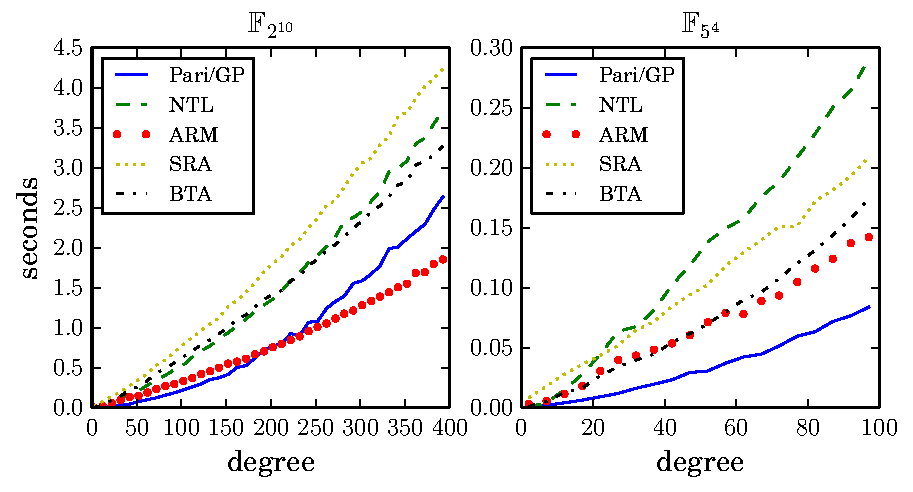
\includegraphics[width=0.55\textwidth]{benchmark}
  \caption{Timings in seconds for $\ff{2^{10}}$ (left) and $\ff{5^4}$
    (right). Abscissa is polynomial degree.}
  \label{fig:benchmarks}
\end{figure}

We used the versions of Pari/GP (v2.7.1) and NTL (v6.1.0) shipped in
the latest Sage distribution (v6.4.1). It should be noted that this is
not the latest NTL version, however we are not aware of any
performance improvements in the latest version (v8.0) concerning root
finding. It is also worth mentioning that the implementation of
polynomials over $\extf$ in Sage 6.4 is backed by the NTL library
(more precisely, by the multi-precision type \texttt{ZZ\_pEX}), thus
the performance of our implementation is essentially to be compared
with NTL's one.

To the best of our knowledge, both Pari/GP and NTL implement the
variant of Cantor-Zassenhaus~\cite{cantor1981} described
in~\cite{GathenS92}. The difference in performances is likely best
explained by the fact that the NTL type \texttt{ZZ\_pEX} is not the
best fit for small characteristic, while Pari/GP optimizes the field
element representation in this case. The fact that our own
implementations performed between the two, and sometimes even better,
shows that these algorithms are practical. However, the observed
differences in performance being so small, they are more likely
attributed to differences in the specific implementation, rather than
to the algorithms themselves.

We conclude that the algorithms reviewed in this paper are of
practical interest for finding polynomial roots in small
characteristic finite fields. In some cases, this in contrast with
what was previously thought, e.g., for ARM. Although general purpose
libraries will probably find no interest in implementing these
algorithms alongside the classical Cantor-Zassenhaus method, they may
turn out to have useful applications in particular finite field
problems.



\section{Conclusion and open problems}

computing $\alpha_i$ in $O(n)$

\paragraph{Aknowledgements} Luca De Feo would like to thank the
Pari/GP team for kindly hosting him in Bordeaux during the preparation
of the paper, and for giving him useful insights on the internals of
Pari/GP. He also thanks Jean-Pierre Flori for his invaluable help
figuring out the gory details of the Sage/NTL interface.

\bibliography{refs}
\bibliographystyle{plain}

\end{document}



% Local Variables:
% ispell-local-dictionary:"american"
% End:


%  LocalWords:  affine subspaces linearized factorizations
%  LocalWords:  iteratively
